\documentclass[
]{beamer}

\usepackage[czech]{babel}
\usepackage[utf8]{inputenc}
\usepackage[T1]{fontenc}
\usepackage{csquotes}
\usepackage{expl3,biblatex}
\usepackage{hyperref}
\usepackage{booktabs}
\usetheme[
  workplace=fi,
]{MU}

\hypersetup{colorlinks,linkcolor=blue,urlcolor=blue}

\title{Verzovací systém git \& GitHub}
\subtitle{Workshop Poznej FI 2024}
\author[Honza Horáček]{Honza Horáček}
\institute[FI MU]{Spolek přátel severské zvěře, Fakulta informatiky, Masarykova univerzita}
\date{17. 2. 2024}
%\subject{}
%\keywords{}
\begin{document}


\begin{frame}[plain]
\maketitle
\end{frame}


\begin{frame}{Letem světem Linuxem}
\begin{itemize}
	\item Login na tabuli, přihlaste se.
	\item Stáhněte si slidy, napoví vám příkazy: \\ \url{https://poznej.fi.muni.cz/git.pdf}
\end{itemize}
\end{frame}

\begin{frame}{Letem světem Linuxem}
\begin{enumerate}
	\item Budeme používat git v terminálu (wtf?!).
	\item Základy práce s terminálem: \\
	prompt, souborový systém, \texttt{ls}, \texttt{cd}, \texttt{Ctrl+C}, man.
	\pause
	\item Textové editory: \texttt{vim}, \texttt{nano}, ...
\end{enumerate}
\end{frame}


\begin{frame}

\includegraphics[width=\textwidth]{images/vim1.png}
\end{frame}


\begin{frame}
\centering

\includegraphics[height=\textheight]{images/vim2.jpg}
\end{frame}


\begin{frame}{Prvotní konfigurace gitu}
Ovládání: \\
\texttt{\$ git <command>} \\
\vspace{1em}

\texttt{\$ git config -{}-global user.name "Honza Horacek"} \\
\pause
Kontrola: \texttt{\$ git config user.name} \\
\pause
\texttt{\$ git config -{}-global user.email "me@apophis.cz"} \\
\texttt{\$ git config -{}-global core.editor vim} :)
\pause

\begin{block}{Pro zvídavé}
\texttt{\$ git config -{}-list} \\
\texttt{\$ git config -{}-help}

Různé úrovně konfigurace: \texttt{-{}-system}, \texttt{-{}-global}, \texttt{-{}-local}
\end{block}
\end{frame}


\begin{frame}{Repozitář}

Repozitář obsahuje verzovaný projekt. Má svou vlastní historii, svoje soubory.

\begin{block}{Repozitář pro tento workshop}
Repozitář s Pythoním programem, který provádí jednoduché textové \uv{šifrovací} operace.
\end{block}

\begin{enumerate}
	\item \texttt{\$ mkdir pficipher}
	\item \texttt{\$ git init}
	\item \texttt{\$ git status}
	\item Šablona kódu: \url{https://poznej.fi.muni.cz/cipher.py}
\end{enumerate}
\end{frame}


\begin{frame}{add, commit, log}
\begin{columns}[T]
\begin{column}{.48\textwidth}
\begin{enumerate}
	\item \texttt{\$ git status}
	\item \texttt{\$ git add cipher.py}
	\item \texttt{\$ git status}
	\item \texttt{\$ git commit}
	\item \texttt{\$ git log}
\end{enumerate}

\end{column}

\begin{column}{.48\textwidth}
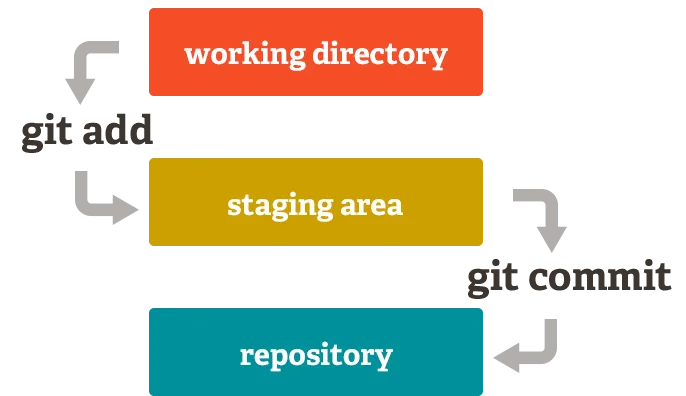
\includegraphics[width=\textwidth]{images/lifecycle.png}
\end{column}
\end{columns}

\pause

\begin{block}{Jak psát commit messages?}
\href{https://gist.github.com/robertpainsi/b632364184e70900af4ab688decf6f53}{Commit Message Guidelines} \\
\href{https://github.com/torvalds/linux}{Ukázka + proč vznikl git}
\end{block}

\begin{block}{Pro zvídavé}
\texttt{\$ git commit -m 'Add template of cipher.py.'} \\
\texttt{\$ git reset}
\end{block}
\end{frame}


\begin{frame}{Jdeme programovat!}
Implementujte nějakou funkci v \texttt{cipher.py}!

Zkuste si pracovat s příkazy:

\begin{itemize}
	\item \texttt{\$ git status}
	\item \texttt{\$ git add}
	\item \texttt{\$ git commit}
	\item \texttt{\$ git log}
	\item \texttt{\$ git reset}
	\item \texttt{\$ git commit -m}
	\item \texttt{\$ git commit -a}
	\item \texttt{\$ git commit -{}-amend}
\end{itemize}

\begin{block}{Může se hodit}
\texttt{\$ git <command> -{}-help}
\end{block}

\end{frame}


\begin{frame}{FAQ}
Rozbil jsem si repozitář...
\end{frame}

\end{document}
